\chapter{Results} \label{ch:results}
The results of the analysis are shown in figs. \ref{fig:dETdEtaOverNpartBy2SumEn}-\ref{fig:comparison}. The error bars in the figures represent the uncertainties propagated from the available data as explained in section \ref{totalET}. In the plots with $\sqrt{s_{NN}}$ as the abscissa, error bars are drawn only on the distribution corresponding to 0-5\% central collision in order to improve the clarity.

Figure \ref{fig:dETdEtaOverNpartBy2SumEn} shows how the transverse energy per nucleon participant pair scales with the total number of nucleon participants in the collisions. As discussed in section \ref{geometry}, $N_{part}$ is generally proportional to the centrality. The results show that the normalized $E_{T}$ does not vary much with $N_{part}$ for more central collisions (higher $N_{part}$ values). It is also seen that the shape of the distribution of this quantity as a function of $N_{part}$ stays roughly the same for different collision energies. Furthermore, the normalized $E_{T}$ is found to increase with the collision energy, mostly when the number of participants is high. Figure \ref{fig:dETdyOverNpartBy2SumEn} is similar to Fig. \ref{fig:dETdEtaOverNpartBy2SumEn} but in rapidity instead of pseudorapidity coordinates. It shows a similar trend, but with an upward shift, of $E_{T}$ distributions.
\afterpage{%
	\begin{figure}[h]
	  \centering
	  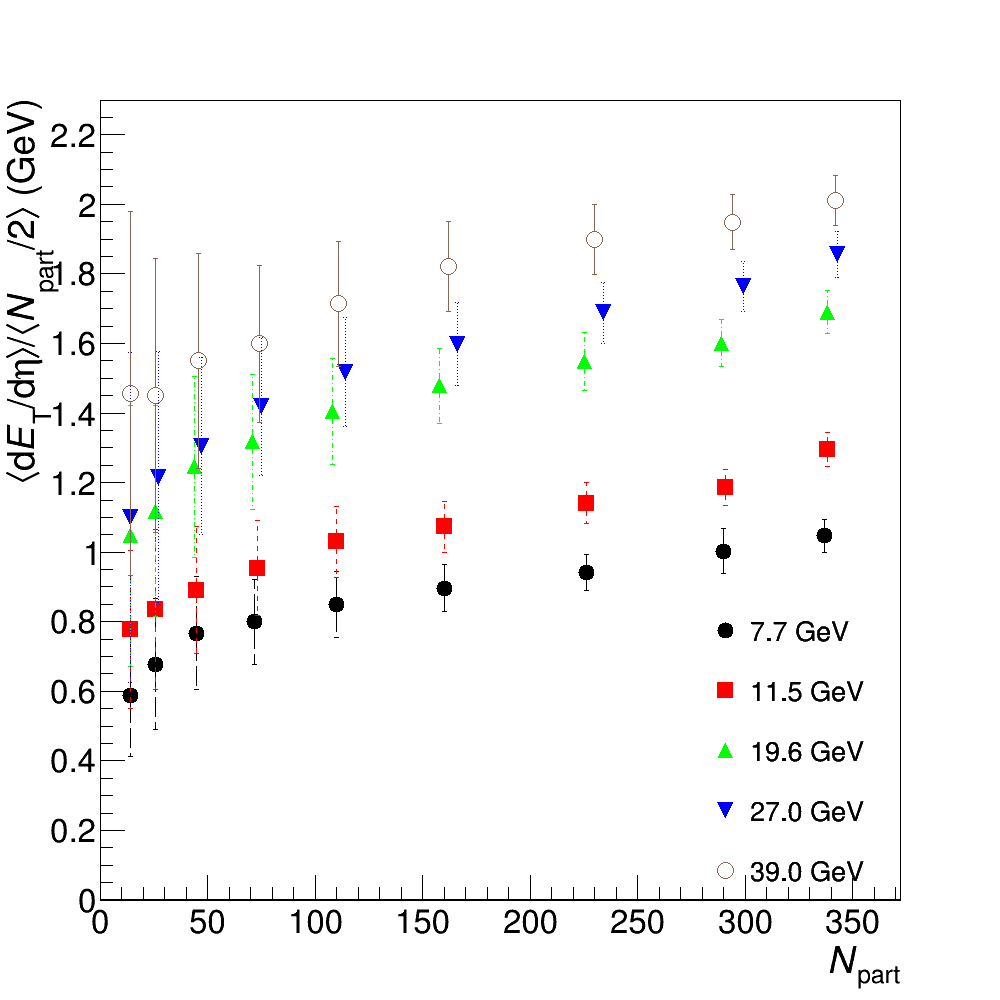
\includegraphics[width=5.5in]{{figures/finalStacked/dETdEtaOverNpartBy2SumEn39.0s}.png}
	  \caption{$(dE_{T}/d\eta)/0.5N_{part}$ at midrapidity as a function of ${N_{part}}$ for different collision energies.}\label{fig:dETdEtaOverNpartBy2SumEn}
	\end{figure}
\clearpage
}
\afterpage{%
	\begin{figure}[h]
	  \centering
	  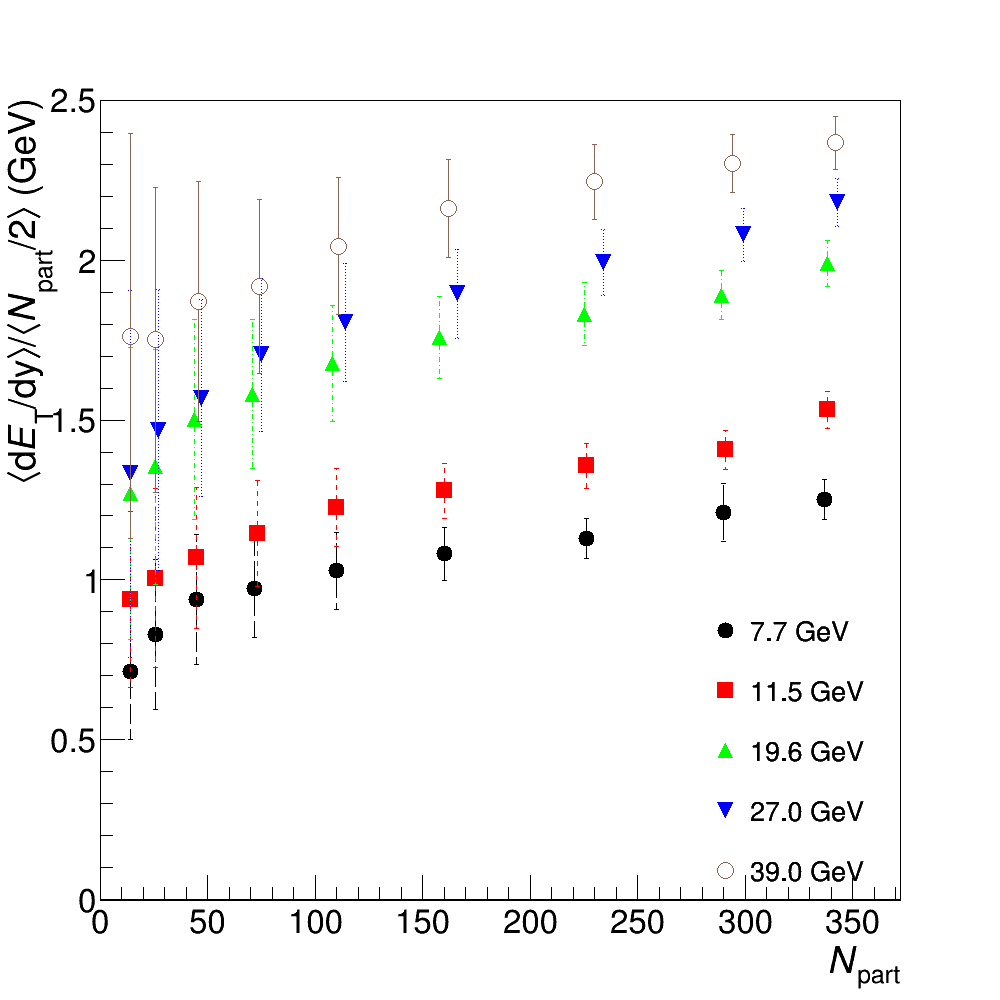
\includegraphics[width=5.5in]{{figures/finalStacked/dETdyOverNpartBy2SumEn39.0s}.png}
	  \caption{$(dE_{T}/dy)/0.5N_{part}$ at midrapidity as a function of ${N_{part}}$ for different collision energies.}\label{fig:dETdyOverNpartBy2SumEn}
	\end{figure}
\clearpage
}

Figure \ref{fig:dETdEtaOverdNchdEtaSumEn} shows the dependence of $E_{T}/N_{ch}$ on the number of nucleon participants. This ratio carries information about the average transverse mass of the final state particles produced from heavy ion collisions, and it has been found to not vary with the collision energy and centrality at RHIC energies \cite{PhysRevC.93.024901}. The results of this analysis show that this ratio remains roughly the same at higher values of $N_{part}$ but tends to grow smaller with decreasing $N_{part}$, albeit within the error bounds. It is also seen to increase with increasing collision energy. Figure \ref{fig:dETdyOverdNchdySumEn} is similar to Fig. \ref{fig:dETdEtaOverdNchdEtaSumEn} but in rapidity instead of pseudorapidity coordinates. The distributions show a similar trend although with some upward shift.
\afterpage{%
	\begin{figure}[h]
	  \centering
	  \includegraphics[width=5.5in]{{figures/finalStacked/dETdEtaOverdNchdEtaSumEn39.0s}.png}
	  \caption{$(dE_{T}/d\eta)/(dN_{ch}/d\eta)$ at midrapidity as a function of ${N_{part}}$ for different collision energies.}\label{fig:dETdEtaOverdNchdEtaSumEn}
	\end{figure}
\clearpage
}

\afterpage{%	
	\begin{figure}[h]
	  \centering
	  \includegraphics[width=5.5in]{{figures/finalStacked/dETdyOverdNchdySumEn39.0s}.png}
	  \caption{$(dE_{T}/dy)/(dN_{ch}/dy)$ at midrapidity as a function of ${N_{part}}$ for different collision energies.}\label{fig:dETdyOverdNchdySumEn}
	\end{figure}
\clearpage
}
%%%%%%%%%% snn plots:
%%%%%%%%%%%%%%%%%%%%%%%%%%%%%%%%%%%%%%%%%%%%%%%%%%%%%%%%%%%	
Figure \ref{fig:dETdEtaOverNpartBy2SumCents} shows the normalized $E_{T}$ as a function of collision energy for all the different collision centralities. This quantity increases with increasing collision energy and centrality while staying within the error bounds of the closest neighboring centralities. The slope of the distribution does not seem to vary a lot between centralities. Figure \ref{fig:dETdyOverNpartBy2SumCents} is similar to Fig. \ref{fig:dETdEtaOverNpartBy2SumCents} but in rapidity instead of pseudorapidity coordinates.
\afterpage{%
	\begin{figure}[h]
	  \centering
	  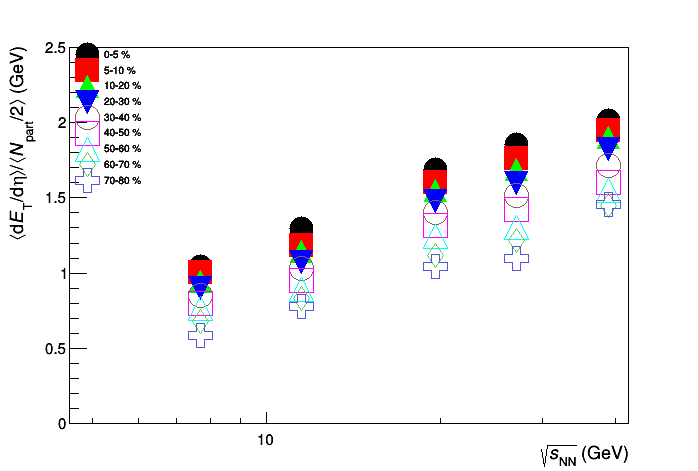
\includegraphics[width=5.5in]{figures/finalStacked/dETdEtaOverNpartBy2SumCent8s.png}
	  %\caption{$(dE_{T}/d\eta)/0.5N_{part}$ at midrapidity as a function of $\sqrt{s_{NN}}$ in logarithmic scale for different centralities. The dashed line represents a power-law fit to the 0-5\% central data in the form $y = ax^{2b}$, where $x$ and $y$ are the placeholders for the quantities in the plot axes. $\chi^{2}/n.d.f$ for the fit was 1.806, and the good-fit parameters were $a = 0.4838 \pm 0.0429$ and $b = 0.2005 \pm 0.01466$. The shaded area represents the uncertainty bounds for the 0-5\% central PHENIX data from \cite{PhysRevC.93.024901}. }\label{fig:dETdEtaOverNpartBy2SumCents}
	  \caption{$(dE_{T}/d\eta)/0.5N_{part}$ at midrapidity as a function of $\sqrt{s_{NN}}$ in logarithmic scale for different centralities.}\label{fig:dETdEtaOverNpartBy2SumCents}
	\end{figure}
\clearpage
}
\afterpage{%
	\begin{figure}[h]
	  \centering
	  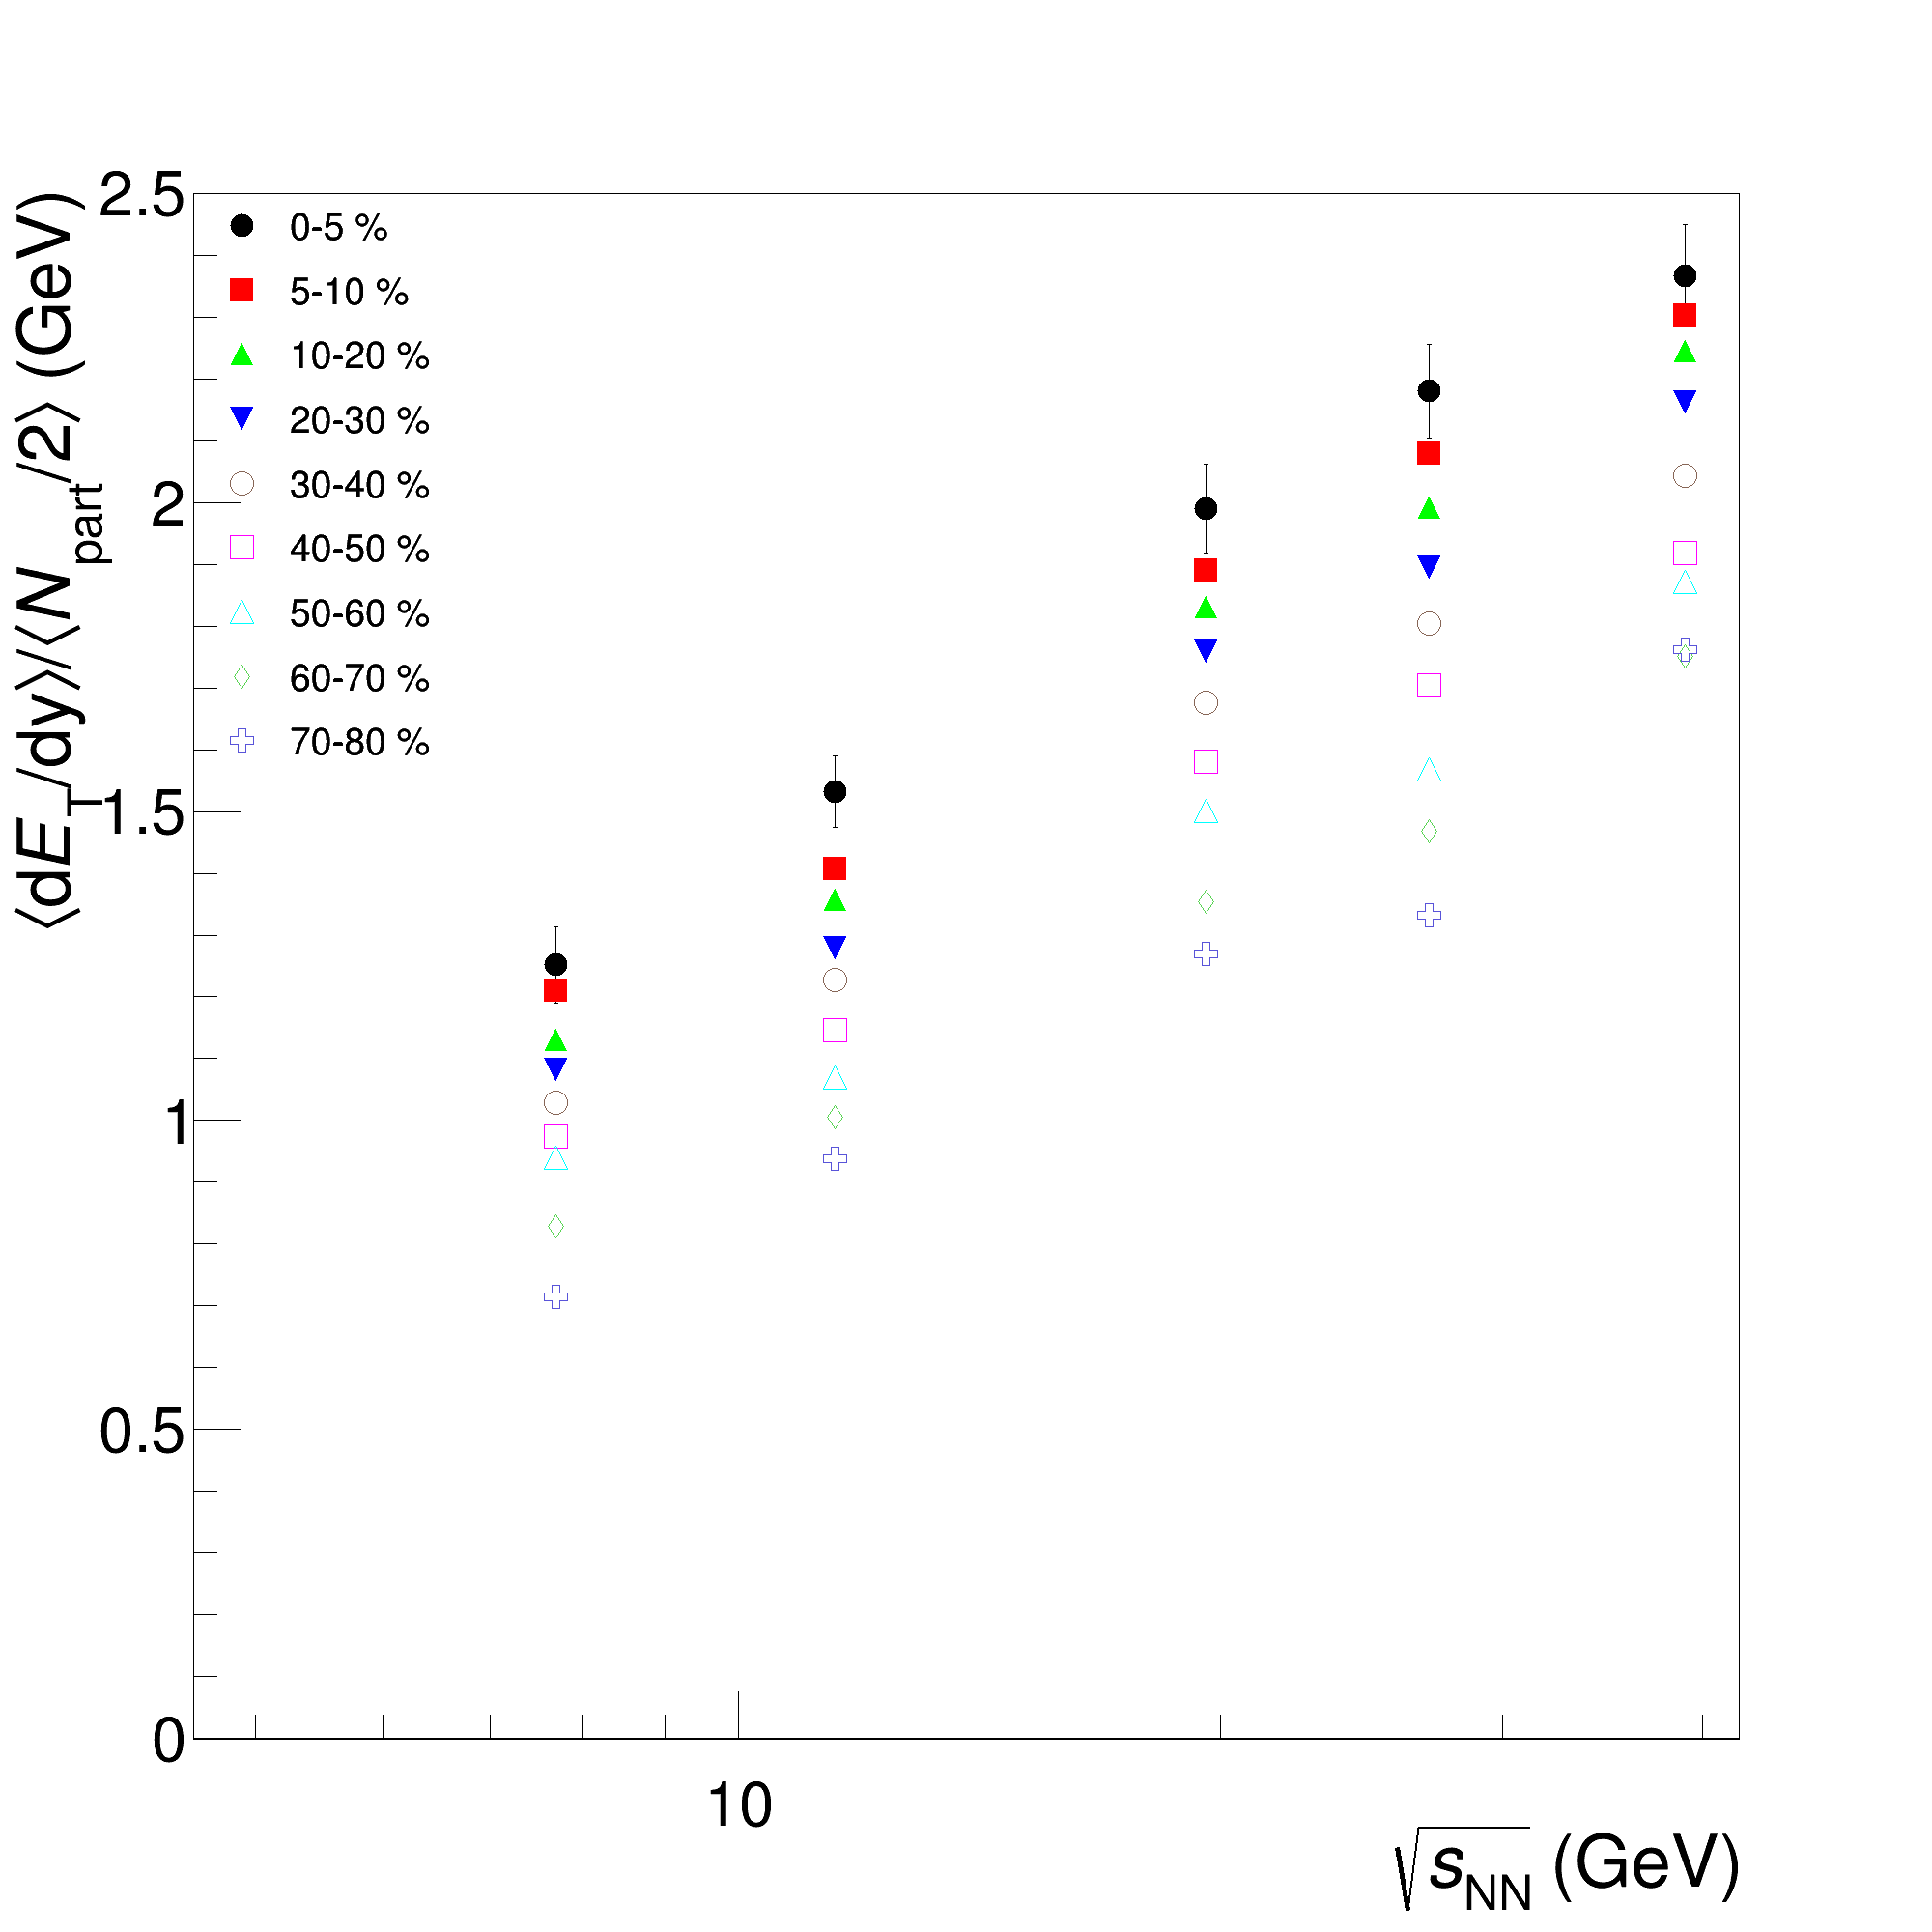
\includegraphics[width=5.5in]{figures/finalStacked/dETdyOverNpartBy2SumCent8s.png}
	  \caption{$(dE_{T}/dy)/0.5N_{part}$ at midrapidity as a function of $\sqrt{s_{NN}}$ for different centralities.}\label{fig:dETdyOverNpartBy2SumCents}
	\end{figure}
\clearpage
}
%%%%%%%%%%%%%%
Figures \ref{fig:dETdEtaOverdNchdEtaSumCents} and \ref{fig:dETdyOverdNchdySumCents} show the dependence of $E_{T}/N_{ch}$ on the collision energy in, respectively, pseudorapidity and rapidity coordinates. The $\sqrt{s_{NN}}$ axis is again in logarithmic scale. The ratio $E_{T}/N_{ch}$ increases with increasing collision energy. The slope of the distributions seem to decrease with increasing centrality for the more central collisions.	The more central collisions also show fluctuations in the way $E_{T}/N_{ch}$ increases as a function of $\sqrt{s_{NN}}$.
	
\afterpage{%
	\begin{figure}[h]
	  \centering
	  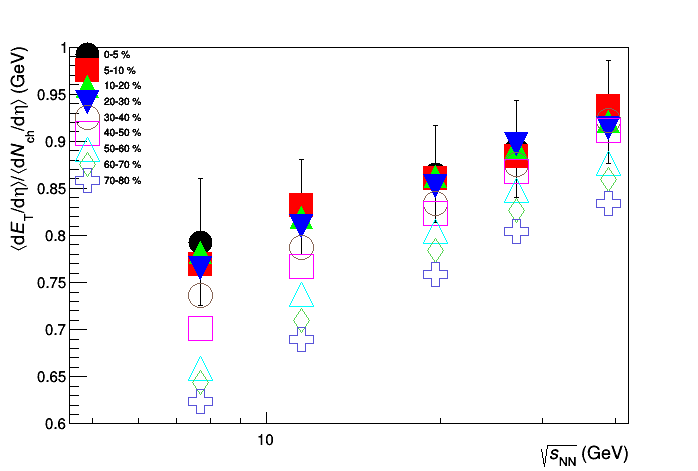
\includegraphics[width=5.5in]{figures/finalStacked/dETdEtaOverdNchdEtaSumCent8s.png}
	  \caption{$(dE_{T}/d\eta)/(dN_{ch}/d\eta)$ at midrapidity as a function of $\sqrt{s_{NN}}$ for different centralities.}\label{fig:dETdEtaOverdNchdEtaSumCents}
	\end{figure}
\clearpage
}	
\afterpage{%
	\begin{figure}[h]
	  \centering
	  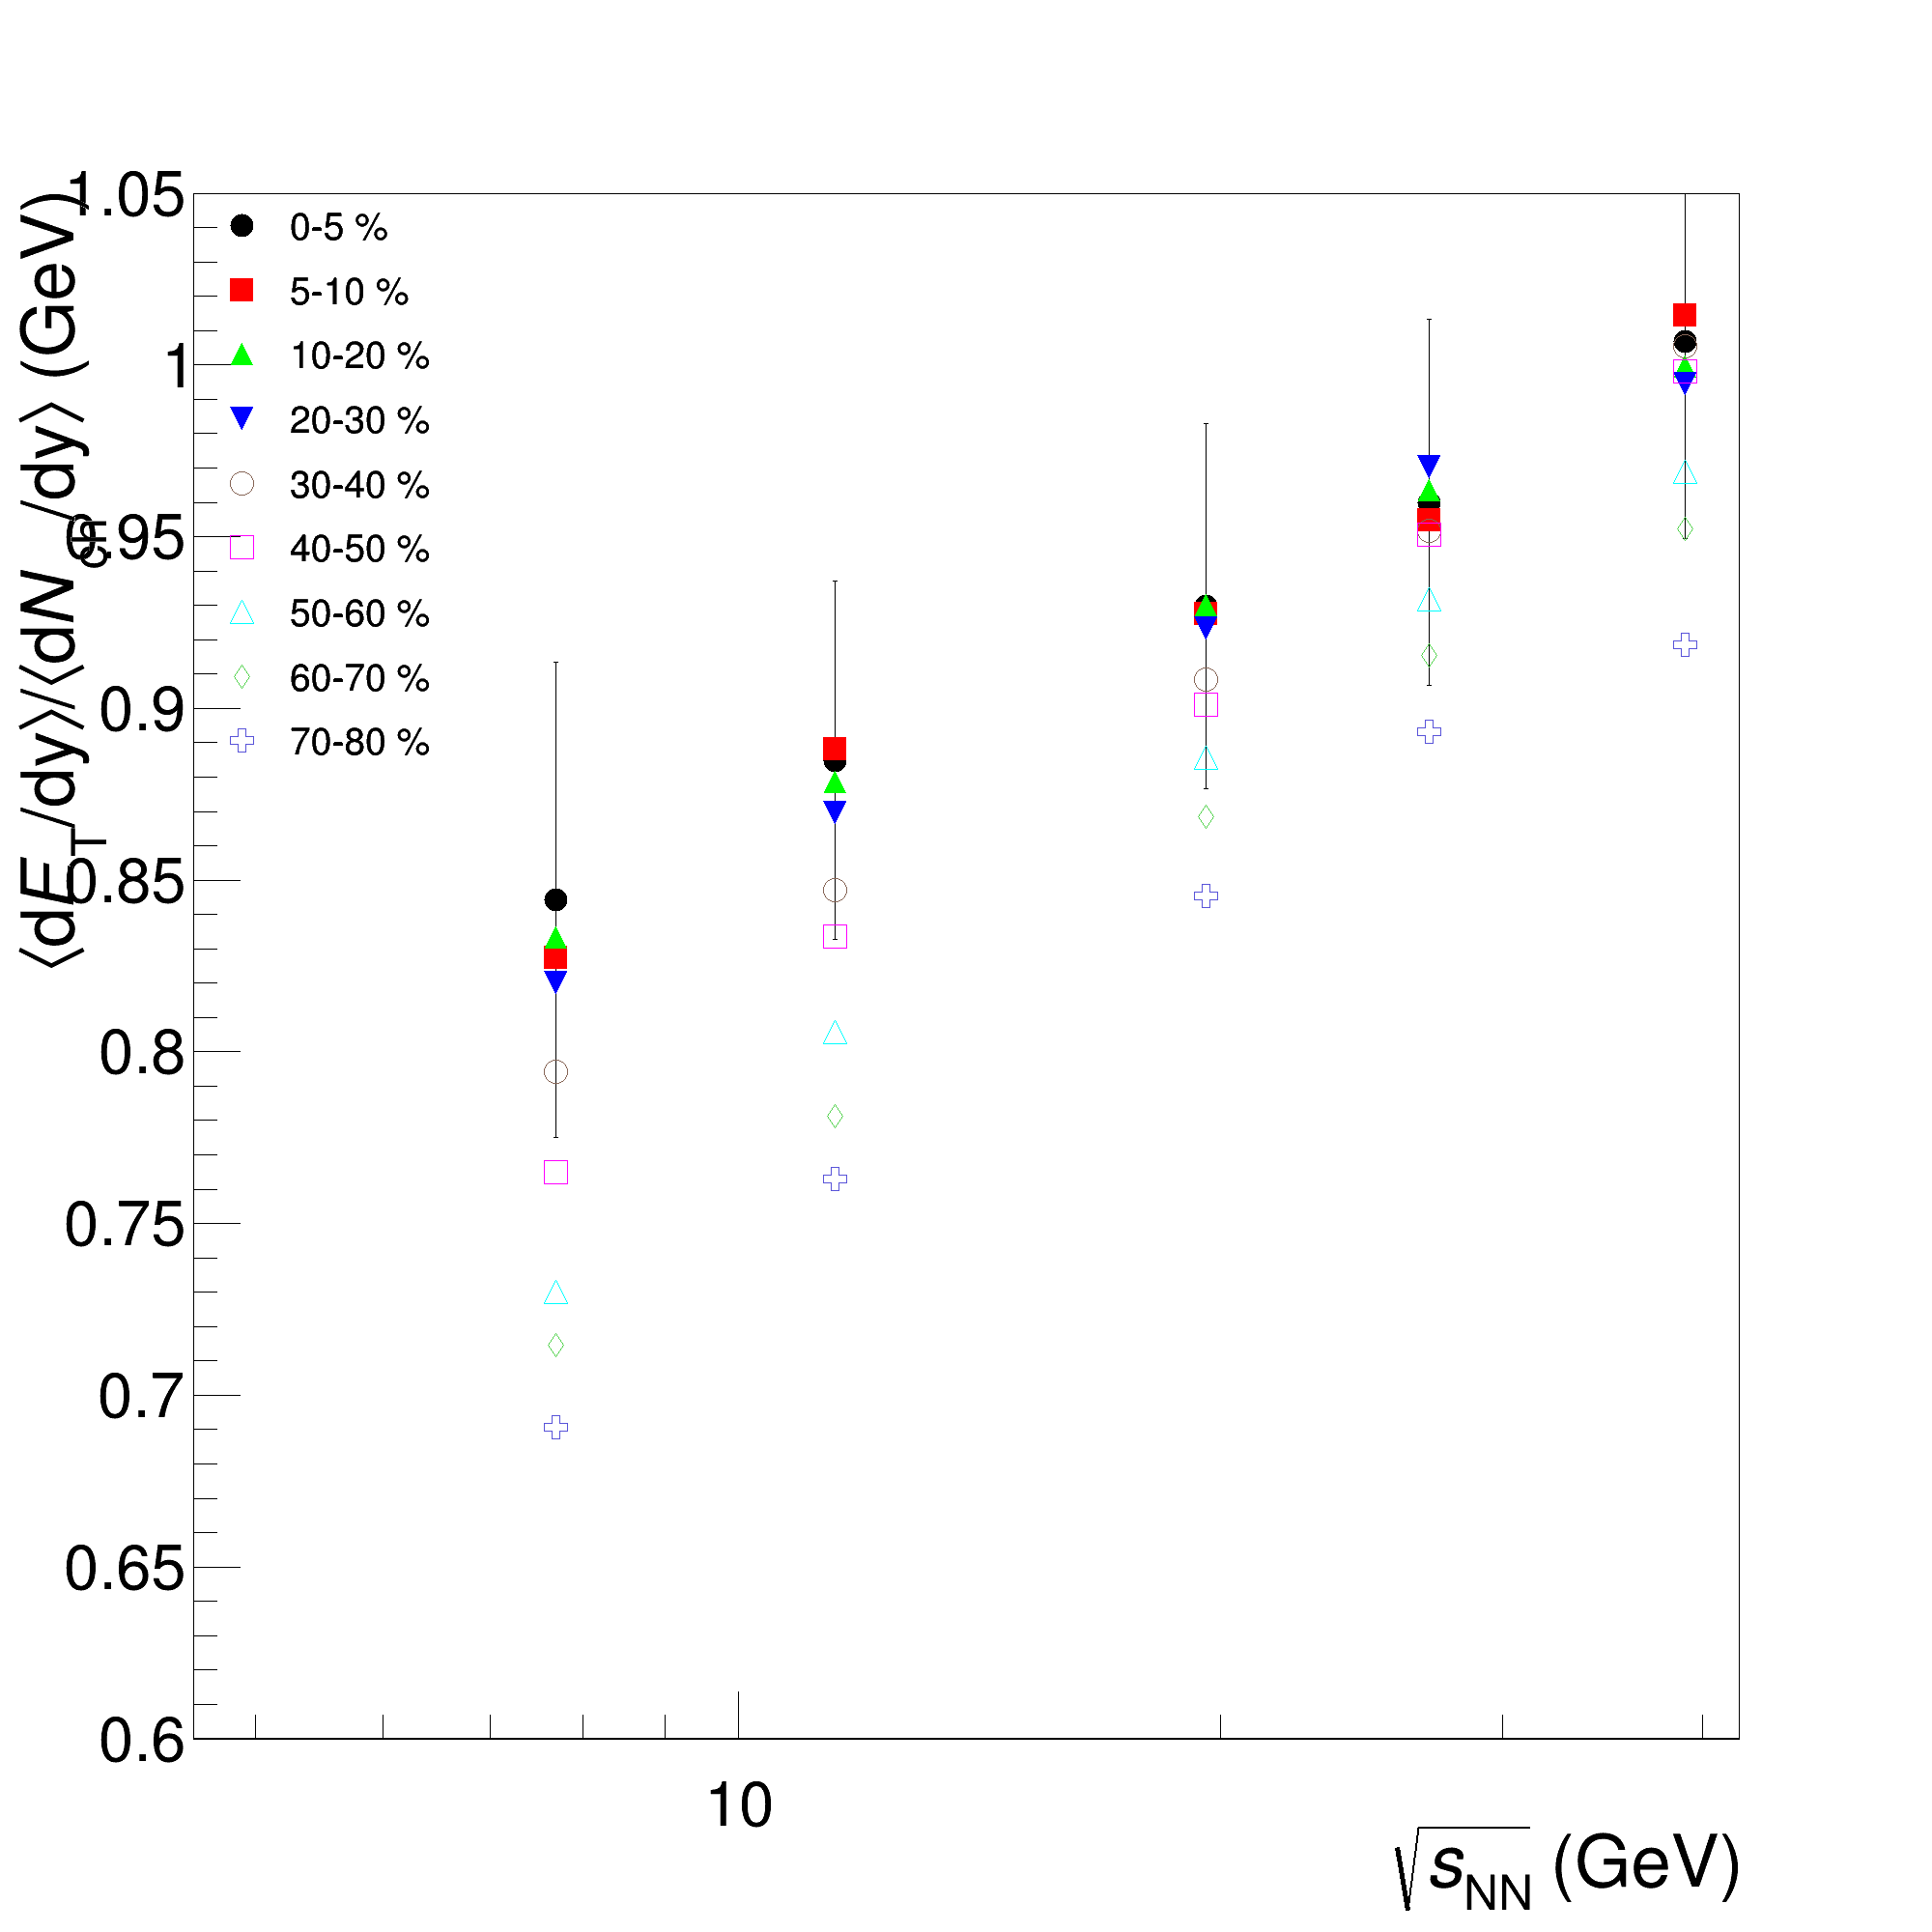
\includegraphics[width=5.5in]{figures/finalStacked/dETdyOverdNchdySumCent8s.png}
	  \caption{$(dE_{T}/dy)/(dN_{ch}/dy)$ at midrapidity as a function of $\sqrt{s_{NN}}$ for different centralities.}\label{fig:dETdyOverdNchdySumCents}
	\end{figure}
\clearpage
}

% comparison with Adare et al.
Figure \ref{fig:comparison} puts the 0-5\% collision results of this analysis in perspective with the result from \cite{PhysRevC.93.024901} based on PHENIX calorimetry. The normalized $E_{T}$ from this analysis is higher than that from PHENIX for all the available collision energies. The $(dE_{T}/dy)/0.5N_{part}$ values for $\sqrt{s_{NN}}$ = 7.7, 19.6, 27, and 39 GeV are found to differ by 2.82, 2.83, 2.37 and 1.67 standard deviations respectively. Since these two measurements are truly independent and the calculated deviations aren't too extreme, this may just reflect a tension between STAR and PHENIX. There may also be a slight effect due to the difference in the rapidity ranges corresponding to the two different measurements, as well as the different sensitivities in the methods to estimate particle compositions and Monte Carlo generators used for corrections. The next step is to make similar comparisons in the collision energy regimes where identified particle spectra are available from both experiments, but that is out of the scope of this thesis.%  The explanation of these differences require a meticulous analysis of the assumptions made by both measurements and is left for future work. 

\afterpage{%
	\begin{figure}[h]
	  \centering
	  \includegraphics[width=4.5in]{figures/PHENIX_comparison2.png}
	  \caption{$\frac{dE_{T}}{d\eta}/0.5N_{part}$ for 0-5\% central collisions at midrapidity as a function of $\sqrt{s_{NN}}$. The PHENIX data are from \cite{PhysRevC.93.024901}. The error bars represent the total statistical and systematic uncertainties.}\label{fig:comparison}
	\end{figure}
\clearpage
}	
	
	
%cnt97kx Send this link to your invitees ... http://whenisgood.net/fndqz2a This is where your results will appear ... http://whenisgood.net/fndqz2a/results/cnt97kx And use this link to edit your event ... http://whenisgood.net/fndqz2a/edit/cnt97kx
